\chapter{Global Basis Time of Maximum}
\label{chap:fixing_t}


\section{Globally shared basis time of maximum}

The investigation of the financial intuition behind a common value for the model parameter $t_{max}$ forms the body of the thesis and the continuation of the research relies on the empirical results which follow this chapter.\footnote{The dataset refers to the 24th of February 2016}In order to evaluate the market data it is possible to exploit the technological tools provided in \eqref{chap:Acdt_framework}.

The algorithm allows to minimize the following quantity globally changing the $t_{max}$ across the different tenor based acdt leaving each $x$ inner model the possibility to minimize its repricing error liberally changing $a_{x}$, $c_{x}$, $d_{x}$:

\begin{equation}
\sqrt{\sum_{i=1}^{n}\left(\sum_{j=1}^{m_{i}}(p_{j}-r_{j})^{2}w_{j} \right)w_{i}}\,,
\label{eq:global_error}
\end{equation}

where:

\begin{itemize}
    \item $p_{j}$ is the j-th market quote;
    \item $r_{j}$ is the j-th model quote;
    \item n is the number of considered acdt models;
    \item m is the tenor dependent number of repriced quotes;
    \item w is the weight (j-th model error or i-th repriced quote).
\end{itemize}

Therefore, the problem can be written as:

\begin{equation*}
\begin{aligned}
& \underset{t_{max}}{min}
& & \sqrt{\sum_{i=1}^{n}(\epsilon_{i}(a_{i},c_{i},d_{i},t_{max}))^{2}w_{i}}\,, \\
\end{aligned}
\end{equation*}

where:

\begin{equation*}
\begin{aligned}
& \underset{a_{i},c_{i},d_{i}}{min}
& & \epsilon_{i}(a_{i},c_{i},d_{i},t_{max})=\sqrt{\sum_{j=1}^{m_{i}}(p_{j}-r_{j}(a_{i},c_{i},d_{i},t_{max}))^{2}w_{j}} \,.\\
\end{aligned}
\end{equation*}

This particular procedure has been applied calibrating the instantaneous basis, the reason is linked with the observation in the chapter \eqref{chap:abcd}, indeed looking at the equation:

\begin{equation}
\int_t^{t+x} s_x(u) \mathrm{d}u = S_x(t) \tau_x(t).
\end{equation}

it is clear that the atomic view appears in the instantaneous form and it allows to compare curve with different tenor which in finite time become a function of the incorporated tenors.

Concluding, despite what has been explained in the introduction the calibration is only not incremental, because (at this step) it makes no sense to define a common time of maximum for the basis with respect to multiple tenors.

\subsection{Empirical results}

Considering both the global error described by \eqref{eq:global_error} which takes a value of 1.84 (sum of root mean square errors below reported) and the correction factors distribution, which is one of the control variable representing the goodness of the calibration in the abcd framework, the results are excellent:

\begin{figure}[H]
\centering
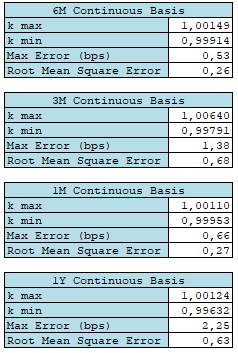
\includegraphics[scale=1]{k_no_inc}
\caption{Correction factors k from not incremental calibration with global $t_{max}$}
\label{fig:k_no_inc_global_t}
\end{figure}

Range of $k$ values is closed to 1 that is the best value because indicates that no corrections are needed.
Moreover, the statistics show an interesting features for the following of the research:

\begin{figure}[H]
\centering
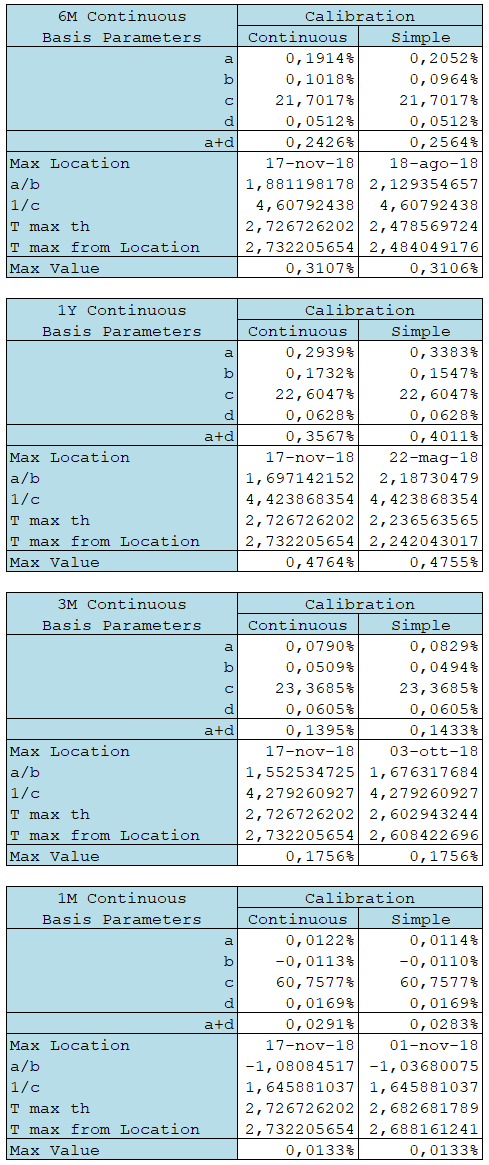
\includegraphics[scale=1]{acdt_Parameters_t}
\caption{Parameters from not incremental calibration with global $t_{max}$}
\label{fig:parameters_no_inc_global_t}
\end{figure}

for 6M, 3M and 1Y the $c$ values are closed to the other:

\begin{figure}[H]
\centering
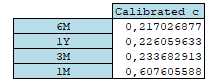
\includegraphics[scale=1]{c_from_calibrated_t}
\caption{c parameters from not incremental calibration with global $t_{max}$}
\label{fig:c_from_calibrated_t}
\end{figure}

and this may indicate that a global shared value of $c$ is a sane idea.


Without considering the noisy 1M:

\begin{figure}[H]
\centering
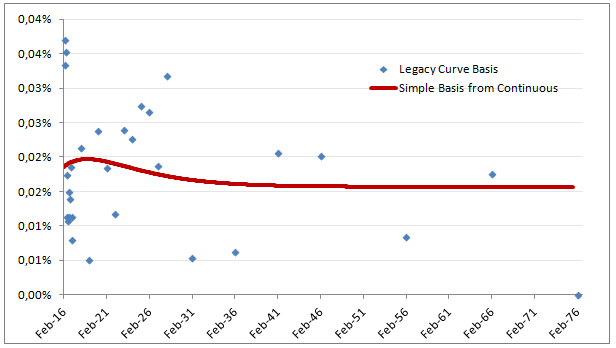
\includegraphics[scale=0.85]{1M_noise}
\caption{1M noisy fitting}
\label{fig:1M_noise}
\end{figure}

the only problem which arises is with respect to the legacy curve, the new basis seems losing fitting on the legacy one, especially on 3M tenor:

\begin{figure}[H]
\centering
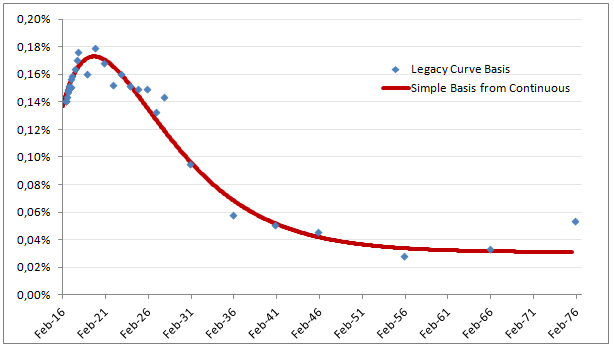
\includegraphics[scale=0.85]{3MLegacy_free}
\caption{3M Legacy vs unconstrained 3M Acdt}
\label{fig:3MLegacy_free}
\end{figure}

\begin{figure}[H]
\centering
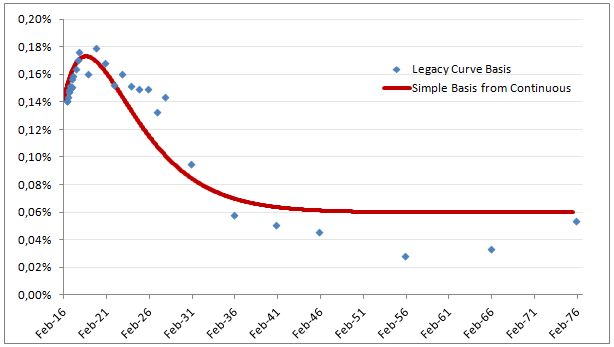
\includegraphics[scale=0.85]{3MLegacy_t}
\caption{3M Legacy vs 3M Acdt (global $t_{max}$)}
\label{fig:3MLegacy_t}
\end{figure}

Anyway, it should not be a problem in the extend which is valid the idea that legacy curve brings with itself more noise than signal with respect to an abcd basis.

%%%%grafici rispetto alla legacy, magari anche rispetto alle legacy incrementali

Moreover, it appears that the matter, encountered in \cite{ametrano_ballabio_mazzocchi}, about the shape of 1M remains:

\begin{figure}[H]
\centering
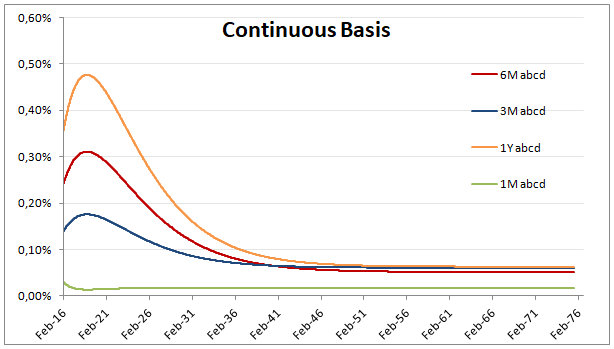
\includegraphics[scale=0.8]{graph_basis_comparison_no_inc}
\caption{Absolute basis from not incremental calibration with global $t_{max}$}
\label{fig:graph_basis_comparison_no_inc}
\end{figure}

However, there are multiple "take away":
\begin{itemize}
    \item the idea of a common $d$ for different tenors is supported by the data and justified by the indifference of long run risk sensibility for the operators because of information lack and incapability to interpret the available one;
    \item the idea of 1M as a slightly bumped ON is justified by the data.
\end{itemize}


Although remembering that the index which points to an acdt basis should be corrected with the $k$ factors in order to perfectly reprice the provided market quotes, it is interesting to look at the "dirty" repricing error for each tenor:

\begin{figure}[H]
\centering
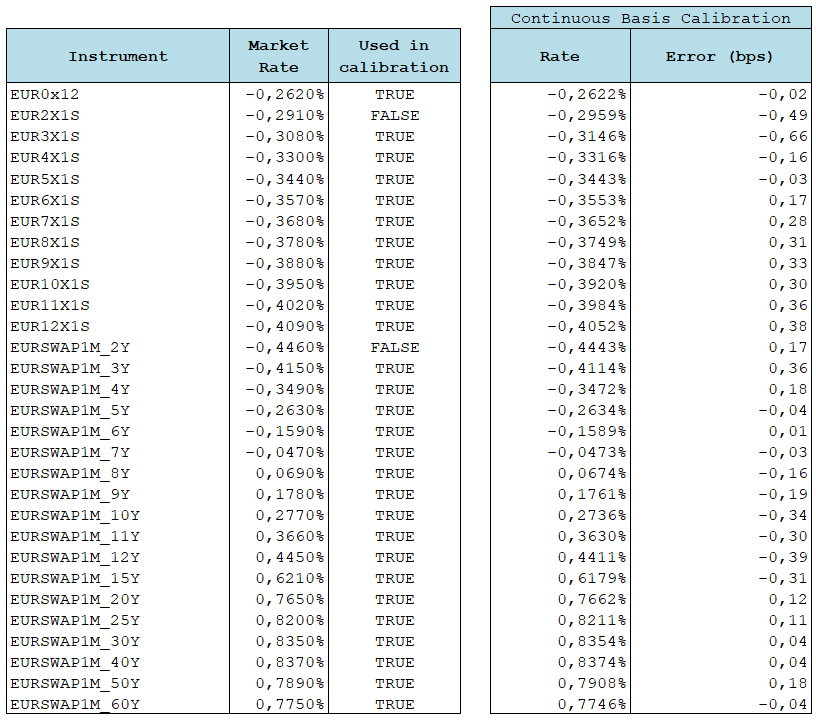
\includegraphics[scale=1]{1Merror_t}
\caption{1M instruments index repricing errors with global $t_{max}$}
\label{fig:1Merror_t}
\end{figure}

\begin{figure}[H]
\centering
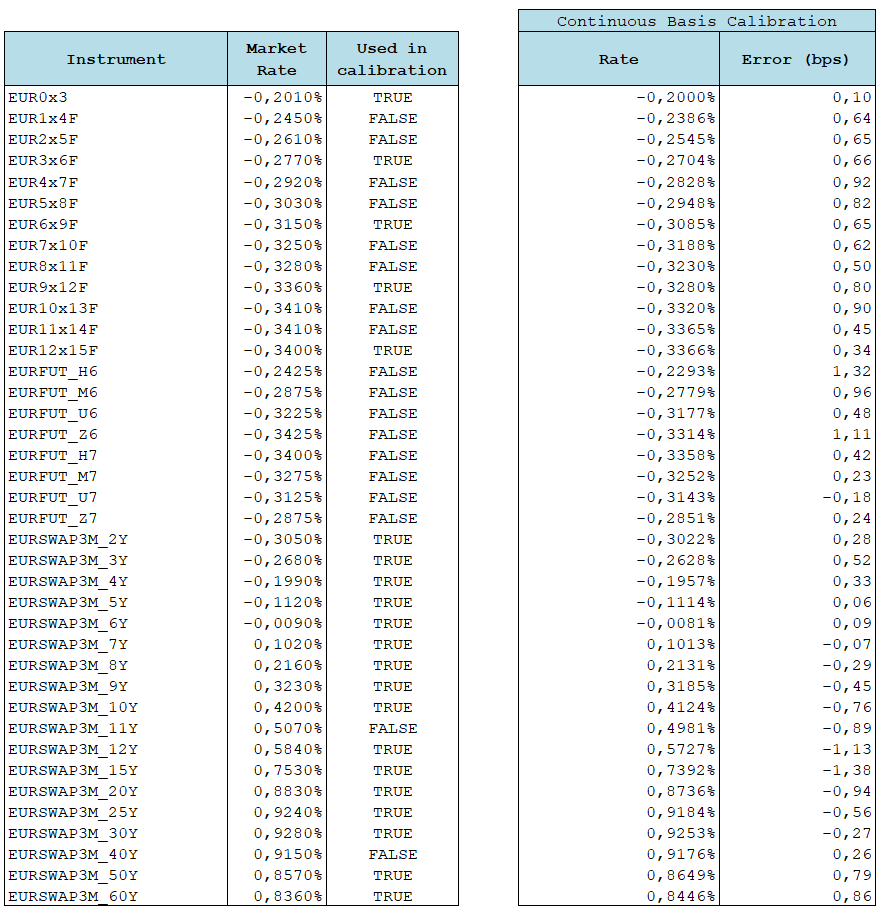
\includegraphics[scale=1]{3Merror_t}
\caption{3M instruments index repricing errors with global $t_{max}$}
\label{fig:3Merror_t}
\end{figure}

\begin{figure}[H]
\centering
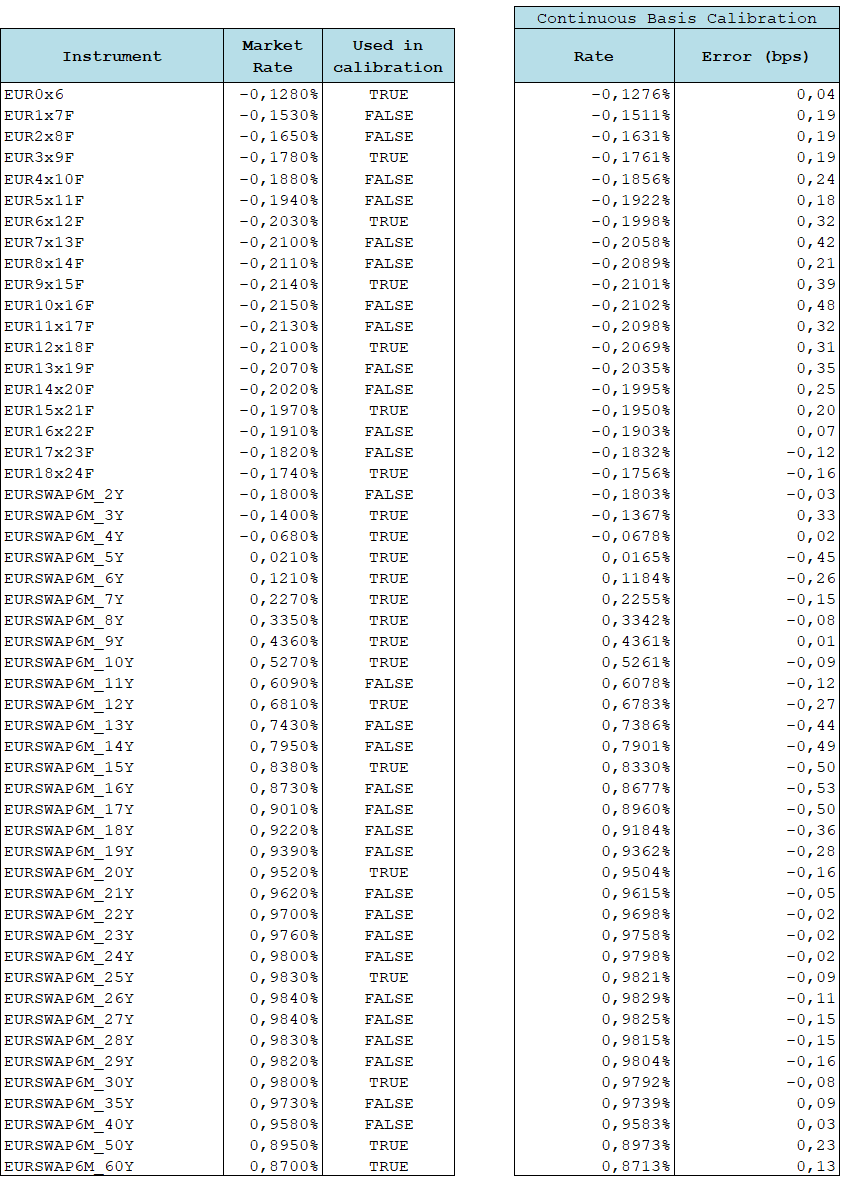
\includegraphics[scale=1]{6Merror_t}
\caption{6M instruments index repricing errors with global $t_{max}$}
\label{fig:6Merror_t}
\end{figure}

\begin{figure}[H]
\centering
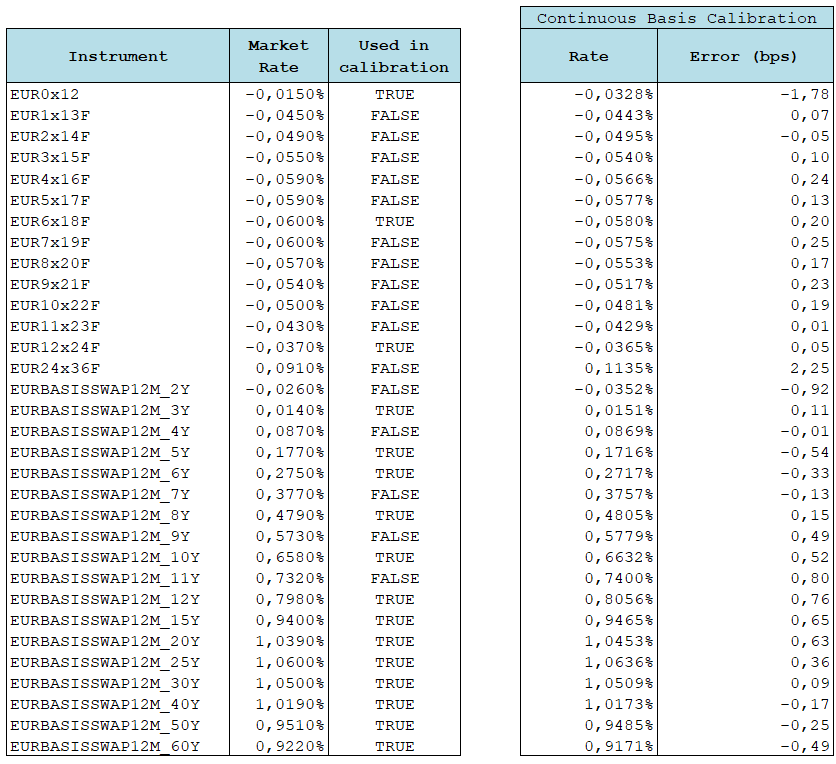
\includegraphics[scale=1]{12Merror_t}
\caption{12M instruments index repricing errors with global $t_{max}$}
\label{fig:12Merror_t}
\end{figure}

Under the hypothesis of a market bid ask spread of 1 basis point all the models but 3M can be considered reliable for an effective employment in a trading desk.
The main findings from this empirical evaluation are:

\begin{itemize}
    \item goodness of fitting which demonstrates the validity of the financial intuition;
    \item without considering the noisy 1M basis on the ON, the $c$ values for the others tenor are closed to a precise value, it follows that it is not an hazard to globally calibrate it and evaluate the associated results.
\end{itemize}

